\documentclass{beamer}
\usepackage[T1,T2A]{fontenc}
\usepackage[utf8]{inputenc}
\usepackage[english,russian]{babel}
\usetheme{Madrid}
\usepackage{csquotes}
\newcommand{\quotes}[1]{``#1''}
%https://www.overleaf.com/help/107-how-to-create-a-basic-slideshow-presentation-in-latex-with-beamer#.V8mZiNFEFqM


\title{Информатика}
\subtitle{Практические занятия}
%\author{Прокшин АН\\taybola@gmail.com}
%\author{\texorpdfstring{Прокшин А.Н.\newline\url{taybola@gmail.com}}{Прокшин Артем Николаевич}}
\institute{ЛЭТИ}

\begin{document}
\begin{frame}
\titlepage
\end{frame}

\begin{frame}
  \tableofcontents
\end{frame}

\section{Порядок сборки ядра}
\frame{\frametitle{Порядок сборки ядра}
\begin{itemize}
\item рекомендуется обновить систему
\begin{quote}
dnf update
\end{quote}
\item переходим в директорию сборки
\begin{quote}cd rpmbuild\end{quote}
\item создаем окружение для сборки пакета
\begin{quote}rpmdev-setuptree\end{quote}

\item скачиваются исходники ядра \begin{quote}dnf download --source kernel\end{quote}
\item устанавливаются зависимости для сборки ядра \begin{quote} dnf builddep kernel-4.8.8-400.fc24.x86\_64\end{quote}
\item скопируем конфиг текущего ядра \begin{quote}cp /boot/config .\end{quote}
\end{itemize}
}
\frame{\frametitle{Порядок сборки ядра}
\begin{itemize}

\item включим требуемые модули
\begin{quote}make menuconfig \end{quote}
\item make modules\_prepare
\item make modules
\item make
\item Установка
\begin{itemize}
\item make modules\_install
\item make install
\end{itemize}

\end{itemize}
}

\section{включение модулей}
\frame{\frametitle{make menuconfig}

\begin{figure}[h]
\center{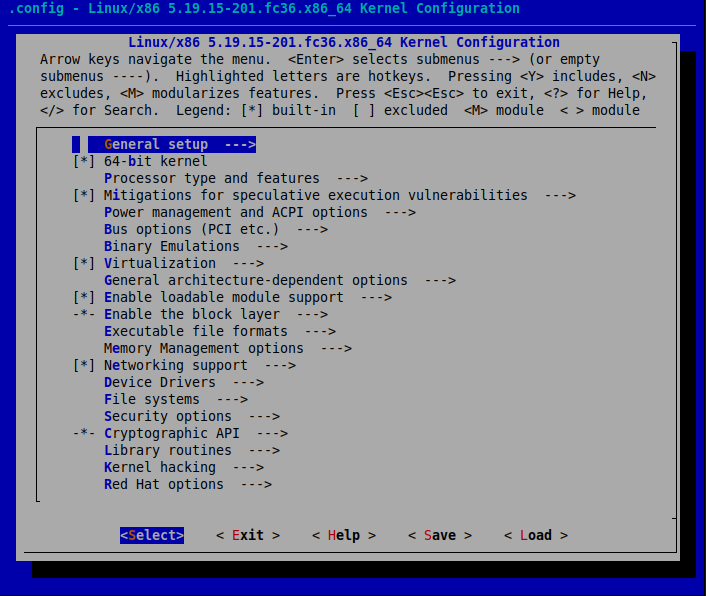
\includegraphics[width=0.8\linewidth]{1.png}}
\caption{начальное окно выбора модулей ядра}
\label{ris:nachalo}
\end{figure}

}

\end{document}

